% I removed the definition of a manifold and moved it in-line for better flow.
% I think it's best to use /emph in definitions to show what's being defined.
% Put periods even in display math!
% For spacing reasons, should use \colon instead of : for functions, e.g. f \colon A \to B.
% Since ker is lowercase, im probably should be also.

\section{Introduction, simplices}\label{905}
%In 18.905, which is the first half of this book, we will cover the following topics:
%\begin{enumerate}
%    \item Singular homology
%    \item CW-complexes
%    \item Basics of category theory
%    \item Homological algebra
%    \item The K\"{u}nneth theorem
%    \item UCT, cohomology
%    \item Cup and cap products, and
%    \item Poincar\'{e} duality.
%\end{enumerate}
We will begin by giving some examples of commonly encountered topological
spaces.
\begin{itemize}
    \item The most basic is \emph{$n$-dimensional Euclidean space}, $\mathbf{R}^n$.
    \item The \emph{$n$-sphere} $S^n=\{x\in \mathbf{R}^{n+1}:|x|=1\}$ is topologized as a subspace of $\mathbf{R}^{n+1}$.
    \item Identifying antipodal points in $S^n$ gives \emph{real projective space} $\mathbf{RP}^n=S^n / (x\sim -x)$, i.e. the space of lines through the origin in $\mathbf{R}^{n+1}$.
    \item Call an ordered collection of $k$ orthonormal vectors an \emph{orthonormal $k$-frame}. The space of orthonormal $k$-frames in $\mathbf{R}^n$ forms the \emph{Stiefel manifold} $V_k(\mathbf{R}^n)$, which is topologized as a subspace of $(S^{n-1})^k$.
    \item Let $x\sim y$ if $x$ and $y$ are $k$-frames with the same span. The \emph{Grassmannian} is the quotient $\mathrm{Gr}_k(\mathbf{R}^n)=V_k(\mathbf{R}^n)/\sim$. In particular, $\mathbf{Gr}_1(\mathbf{R}^n) = \mathbf{RP}^{n-1}$.
\end{itemize}
The above are all \emph{manifolds}, which are Hausdorff spaces locally homeomorphic to Euclidean space. Aside from $\mathbf{R}^n$ itself, the preceding examples are also compact. Such spaces exhibit a hidden symmetry, which is the culmination of 18.905: Poincar\'{e} duality.

As the name suggests, the central aim of algebraic topology is the usage of algebraic tools to study topological spaces. A common technique is to probe topological spaces via maps to them. In different ways, this approach gives rise to singular homology and homotopy groups. We now detail the former; the latter takes stage in 18.906.
\begin{definition}
For $n\geq 0$, the \emph{standard $n$-simplex} $\Delta^n$ is the convex hull of the standard basis $\{e_0,\cdots,e_n\}$ in $\mathbf{R}^{n+1}$. More explicitly,
$$\Delta^n = \left\{\sum t_i e_i : \sum t_i = 1, t_i\geq 0\right\}\subseteq\mathbf{R}^{n+1}.$$
The $t_i$ are called barycentric coordinates.
\end{definition}
\begin{figure}[H]
	\centering
	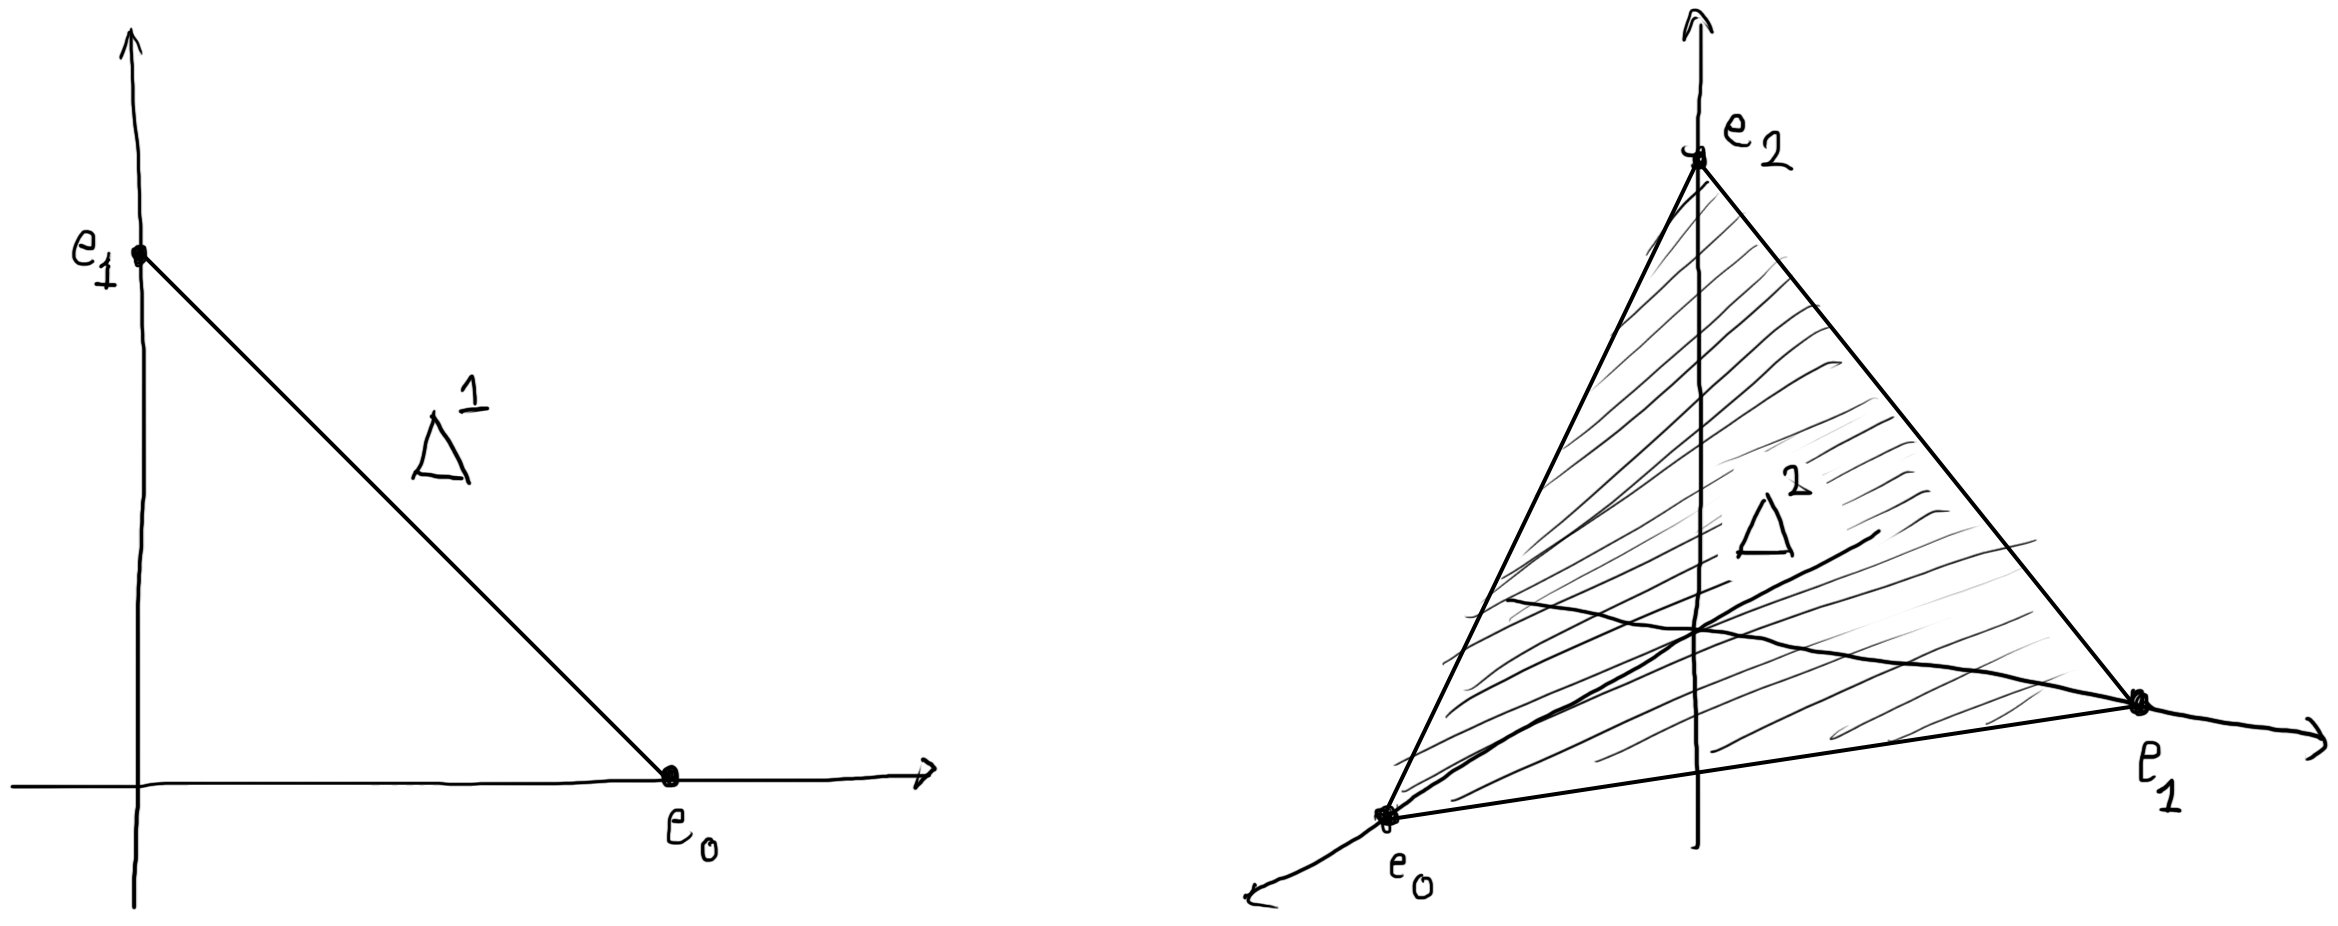
\includegraphics[width=0.9\linewidth]{assets/L01/01-standard-simplices}
	\caption{The standard 1-simplex and 2-simplex.}
	\label{fig:01-standard-simplices}
\end{figure}
We will write $i$ in lieu of $e_i$ to refer to the vertices of $\Delta^n$. The standard simplices are related by face inclusions $d^i\colon \Delta^{n-1} \to \Delta^{n}$ for $0\leq i \leq n$, where $d^i$ misses the vertex $i$.
\begin{figure}[H]
	\centering
	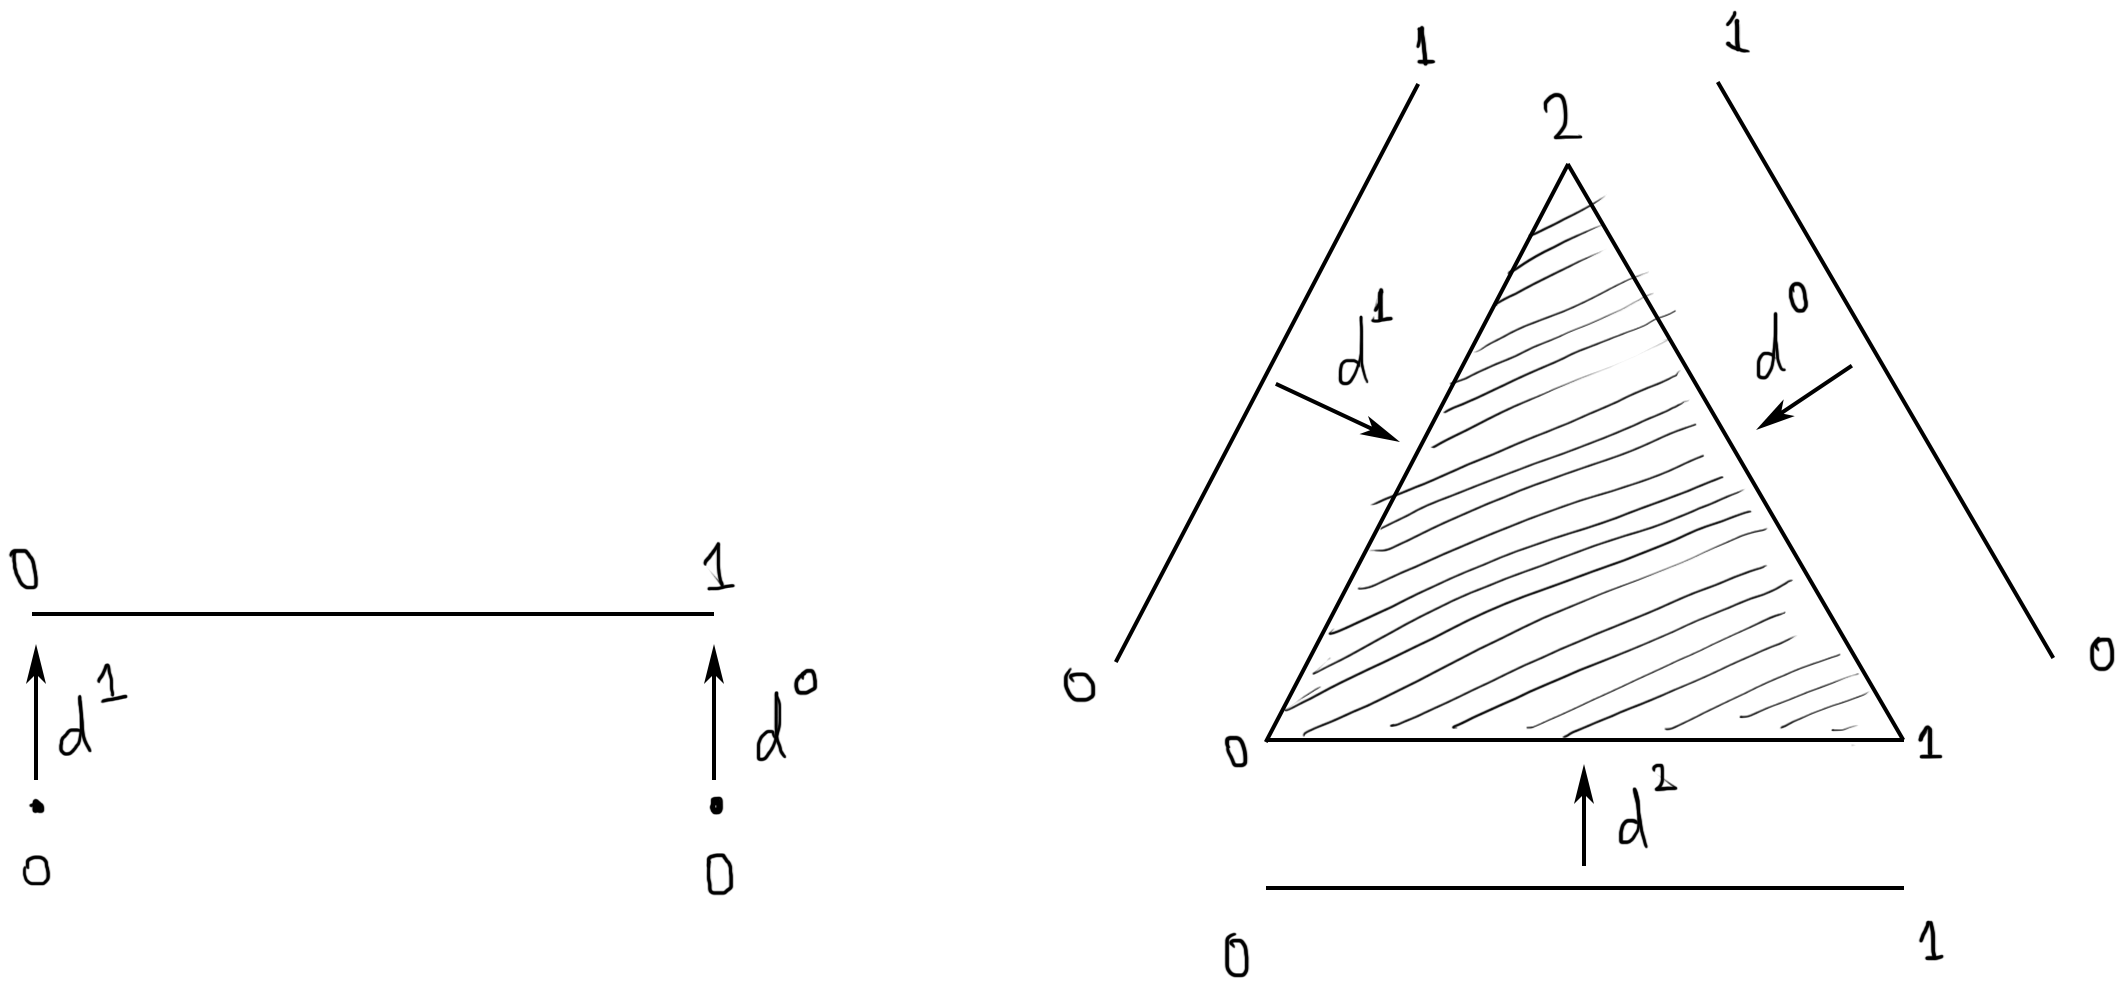
\includegraphics[width=0.9\linewidth]{assets/L01/01-face-inclusions}
	\caption{The face inclusions for $n=1$ (left) and $n=2$ (right).}
	\label{fig:01-face-inclusions}
\end{figure}
\begin{definition}
Let $X$ be any topological space. A \emph{singular $n$-simplex} in $X$ is a continuous map $\Delta^n\to X$. Denote by $\mathrm{Sin}_n(X)$ the set of all $n$-simplices in $X$. This seems like a rather bold construction to make, as $\mathrm{Sin}_n(X)$ is huge. Nonetheless, we will soon make it even larger.
\end{definition}
\begin{figure}[H]
	\centering
	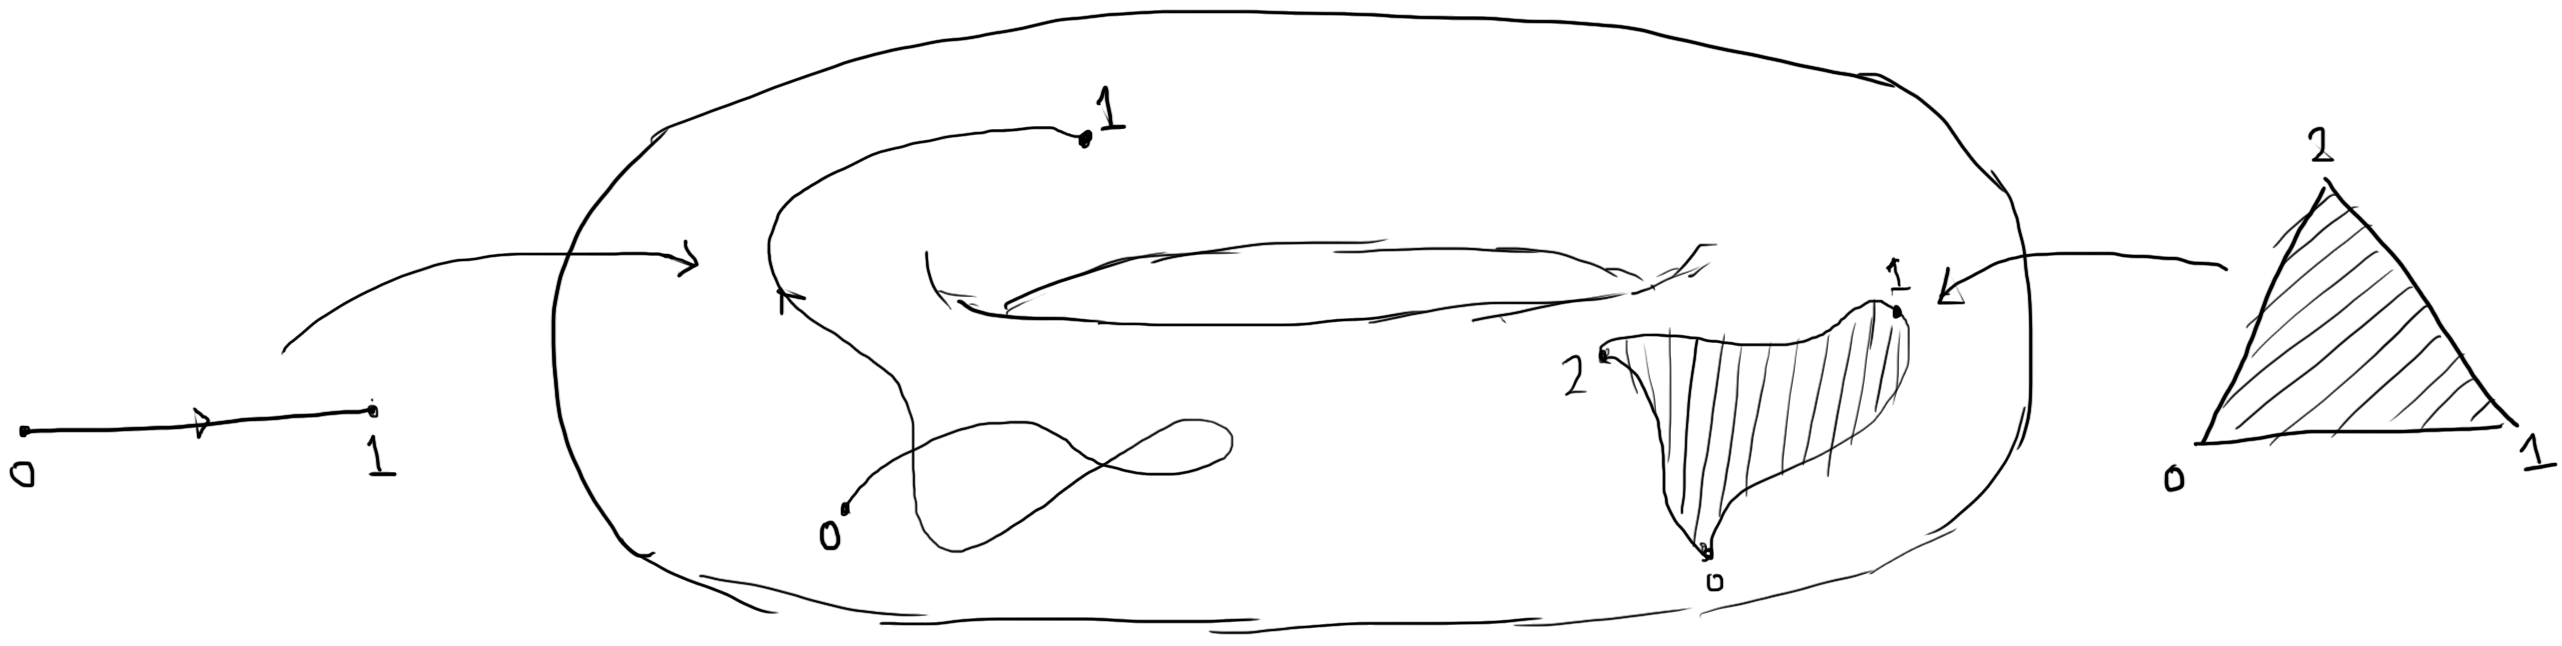
\includegraphics[width=\linewidth]{assets/L01/01-simplices-on-torus}
	\caption{A 1-simplex and a 2-simplex in the torus.}
	\label{fig:01-simplices-on-torus}
\end{figure}

For $0\leq i \leq n$, precomposition by the face inclusion $d^i$ produces a map $d_i\colon \Sin_n(X)\to\Sin_{n-1}(X)$ sending $\sigma\mapsto\sigma\circ d^i$, which is the $i$th face of $\sigma$. This allows us to make sense of the ``boundary'' of a simplex, and we are particularly interested in simplices for which that boundary vanishes.
\begin{figure}
	\centering
	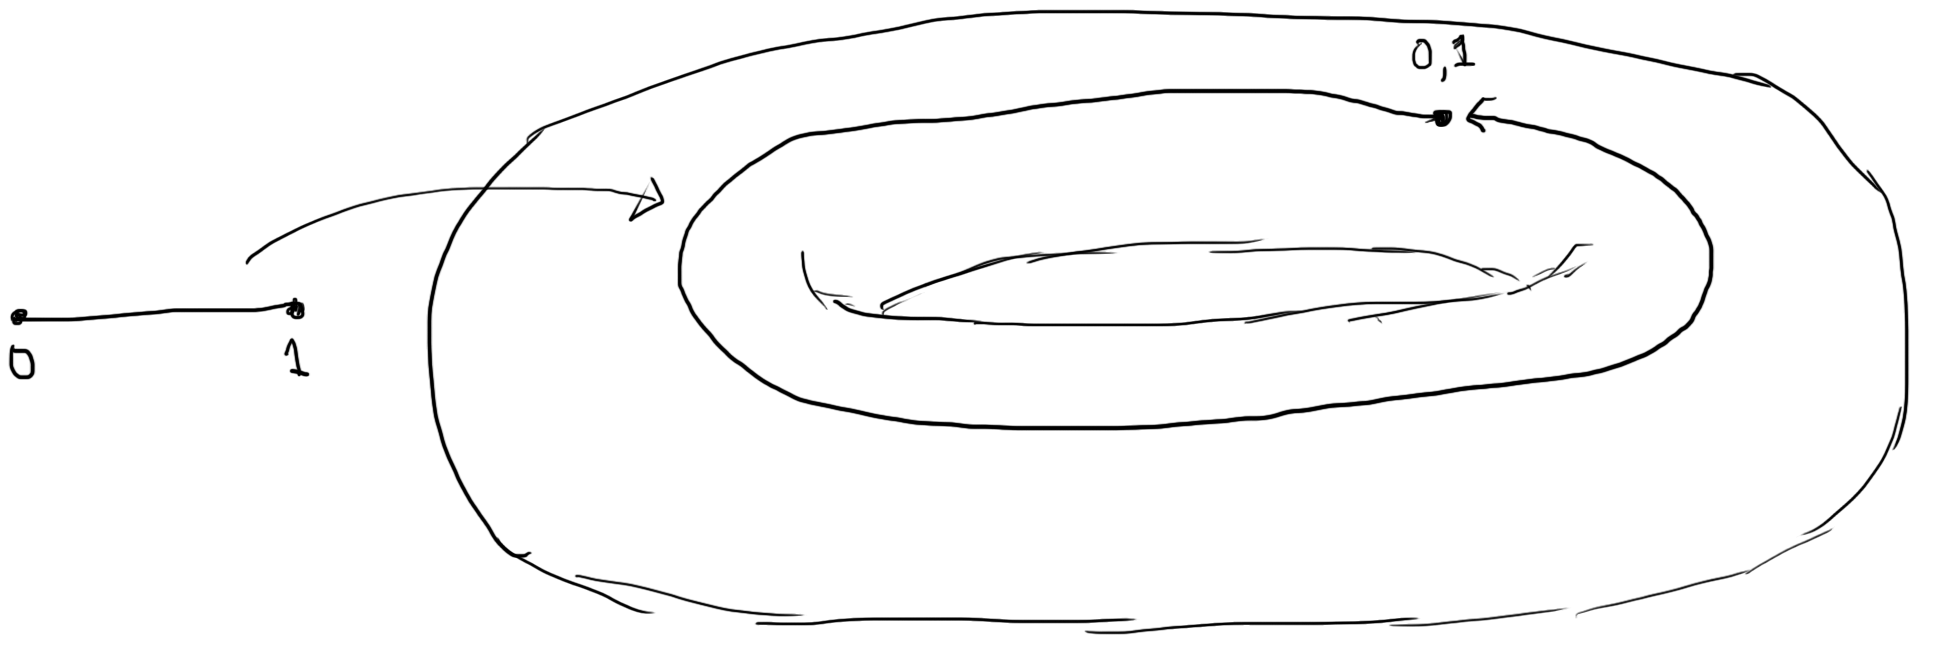
\includegraphics[width=0.7\linewidth]{assets/L01/01-torus-simplex-around-hole}
	\caption{A 1-simplex around the hole in the torus.}
	\label{fig:01-torus-simplex-around-hole}
\end{figure}
For example, if $\sigma$ is a 1-simplex that goes around the hole in a torus $T$ as in Figure \ref{fig:01-torus-simplex-around-hole}, then $d_1\sigma = d_0\sigma$. To express that the boundary vanishes, we want to write $d_0\sigma - d_1\sigma=0$, but this difference is no longer a simplex. To accommodate such formal sums, we will enlarge $\mathrm{Sin}_n(X)$ further by considering the free abelian group it generates.
\begin{definition}
The abelian group $S_n(X)$ of \emph{singular $n$-chains} in $X$ is the free abelian group generated by $n$-simplices
$$S_n(X) = \mathbf{Z}\Sin_n(X).$$
    Its elements are finite linear combinations, i.e. formal sums
    $$\sum_{i\in\text{finite set}}a_i\sigma_i$$
    where $a_i\in\mathbf{Z}$ and $\sigma_i \in \Sin_n(X)$. If $n<0$, say that $S_n(X)=0$. Now, define
$$\partial\colon \Sin_n(X)\to S_{n-1}(X),$$
$$\partial\sigma = \sum_{i=0}^n(-1)^i d_i\sigma.$$
This extends to a homomorphism $\partial \colon S_n(X) \to S_{n-1}(X)$ by additivity.
\end{definition}
We use this homomorphism to obtain something more tractable than the entirety of $S_n(X)$. First we restrict our attention to chains with vanishing boundary.
\begin{definition}
An \emph{$n$-cycle} in $X$ is an $n$-chain $c$ with $\partial c = 0$. Denote $Z_n(X) = \ker(S_n(X)\xrightarrow{\partial}S_{n-1}(X))$.
\end{definition}
For example, with $\sigma$ on the torus described before, $\sigma\in Z_1(X)$
since $\partial \sigma = d_0\sigma - d_1\sigma = 0$.
\begin{theorem}
    Any boundary is a cycle, i.e., $B_n(X) :=
    \mathrm{Im}(\partial:S_{n+1}(X)\to S_n(X))\subseteq Z_n(X)$.
\end{theorem}
\begin{exercise}\label{exer:simplicialidentities}
    Deduce the above theorem by proving the following statements.
    \begin{enumerate}
	\item An order-preserving map $\phi:[n]\to[m]$ extends to an affine map
	    $\phi^\ast:\Delta^n\to \Delta^m$. Give an explicit formula for
	    $\phi^\ast$.
	\item Prove that any order-preserving map factors uniquely as the
	    composite of an order-preserving surjection followed by an
	    order-preserving injection.
	\item Let $d^j:[n-1]\to [n]$ be the order-preserving injection omitting
	    $j$ as a value. Prove that an order-preserving injection
	    $\phi:[n-k]\to[n]$ is uniquely a composition of the form $d^{j_k}
	    d^{j_{k-1}}\cdots d^{j_1}$ with $0\leq j_1<j_2<\cdots<j_k\leq n$.
	    Define the $j_i$'s in terms of $\phi$. Verify the straightening
	    rule
	    $$d^id^j = d^{j+1} d^i \text{ if }i\leq j.$$
	\item Let $s^i:[n+1]\to [n]$ be the order-preserving surjection
	    repeating the value $i$. Show that any order-preserving surjection
	    $\phi:[m]\to [n]$ is uniquely a composition of the form
	    $(s^n)^{i_n}(s^{n-1})^{i_{n-1}}\cdots(s^0)^{i_0}$ by describing the
	    $i_j$'s in terms of $\phi$. Verify a straightening rule for the
	    composite $s^i s^j$.
	\item Verify a straightening rule for $s^i d^j$.
	\item Write down the straightening rules for the induced maps $d_i =
	    (d^i)^\ast:\Sin_n(X)\to \Sin_{n-1}(X)$ and $s_i =
	    (s^i)^\ast:\Sin_m(X)\to \Sin_{m+1}(X)$. Use these to verify that
	    $\partial^2 = 0:S_n(X)\to S_{n-2}(X)$.
	\item Let $f:X\to Y$ be a continuous map. This induces a map
	    $f_\ast:\Sin_n(X)\to \Sin_n(Y)$. Show that the $f_\ast$ assemble to
	    give a map of simplicial sets, i.e., show that the maps $f_\ast$
	    commute with the maps induced by order-preserving maps $\phi:[m]\to
	    [n]$.
    \end{enumerate}
\end{exercise}

With the preceding, we are prepared to define singular homology.
\begin{definition}
The \emph{$n$th singular homology group} of $X$ is:
    $$ H_n(X) = Z_n(X)/B_n(X) = \frac{\ker(\partial:S_n(X)\to S_{n-1}(X))}{\mathrm{im}(\partial:S_{n+1}(X)\to S_n(X))}.$$
\end{definition}
Both $Z_n(X)$ and $B_n(X)$ are free abelian groups because they are subgroups of the free abelian group $S_n(X)$, but the quotient $H_n(X)$ isn't necessarily free. While $Z_n(X)$ and $B_n(X)$ are uncountably generated, $H_n(X)$ is finitely generated for the spaces we are interested in. If $T$ is the torus for example, then $H_1(T) \cong \mathbf{Z} \oplus \mathbf{Z}$ and $\sigma$ as described previously is one of the two generators.
